\documentclass[landscape]{article}
\usepackage[landscape,margin=0.7in]{geometry}
\usepackage{pgfplots}
\usepackage{tikz}
\pgfplotsset{compat=1.18}

\begin{document}
\pagestyle{empty}

\begin{figure}
    \centering
    \begin{tikzpicture}
        \begin{axis}[
            title={\Large Random Strategy - Step 2: Middle Boarding Phase (t = 10 minutes)},
            xlabel={Seat Column},
            ylabel={Row Number},
            xticklabels={A,B,C,D,E,F},
            ytick={1,2,3,4,5,6,7,8,9,10,11,12,13,14,15,16,17,18,19},
            xtick={0,1,2,3,4,5},
            xmin=-0.5,
            xmax=5.5,
            ymin=0.5,
            ymax=19.5,
            y dir=reverse,
            enlargelimits=false,
            axis on top,
            width=0.9\textwidth,
            height=0.4\textheight,
            colorbar,
            colormap={boarding}{
                color(0)=(white);
                color(0.5)=(yellow);
                color(1)=(purple)
            },
            colorbar style={
                title={Status},
                ytick={0,0.5,1},
                yticklabels={Empty,Boarding,Seated},
            },
            point meta min=0,
            point meta max=1
        ]
            
        % Initialize seats for middle boarding phase
        \addplot[matrix plot, mesh/cols=6, point meta=explicit] table [meta=C] {
            x y C
            0 1 1
            1 1 0
            2 1 0.5
            3 1 1
            4 1 0
            5 1 0.5
            0 2 0
            1 2 1
            2 2 0
            3 2 0
            4 2 0.5
            5 2 0
            0 3 1
            1 3 1
            2 3 0.5
            3 3 0
            4 3 0
            5 3 1
            0 4 0
            1 4 1
            2 4 1
            3 4 0
            4 4 0.5
            5 4 1
            0 5 0.5
            1 5 0
            2 5 0
            3 5 1
            4 5 1
            5 5 0
            0 6 0
            1 6 0.5
            2 6 0
            3 6 0
            4 6 0
            5 6 1
            0 7 1
            1 7 0
            2 7 1
            3 7 0.5
            4 7 0
            5 7 0
            0 8 0
            1 8 0
            2 8 0
            3 8 0
            4 8 1
            5 8 0.5
            0 9 1
            1 9 0.5
            2 9 0
            3 9 0
            4 9 1
            5 9 1
            0 10 0
            1 10 0
            2 10 1
            3 10 0.5
            4 10 0
            5 10 0
            0 11 0.5
            1 11 0
            2 11 0
            3 11 1
            4 11 0
            5 11 1
            0 12 1
            1 12 0
            2 12 0.5
            3 12 0
            4 12 1
            5 12 0
            0 13 0
            1 13 1
            2 13 0
            3 13 1
            4 13 0.5
            5 13 0
            0 14 0.5
            1 14 0
            2 14 1
            3 14 0
            4 14 1
            5 14 0
            0 15 0
            1 15 1
            2 15 0.5
            3 15 0
            4 15 0
            5 15 1
            0 16 1
            1 16 1
            2 16 0
            3 16 0.5
            4 16 0
            5 16 0
            0 17 0
            1 17 0
            2 17 1
            3 17 1
            4 17 0.5
            5 17 0
            0 18 0.5
            1 18 0
            2 18 0
            3 18 0
            4 18 1
            5 18 0
            0 19 1
            1 19 0.5
            2 19 0
            3 19 0
            4 19 0
            5 19 1
        };
        
        % Draw aisle line
        \draw[black, thick, dashed] (axis cs:2.5,0.5) -- (axis cs:2.5,19.5);
        
        % Time indicator
        \node[font=\Large] at (axis cs:2.5,20.5) {t = 10 minutes};
        
        % Legend for random strategy
        \node[draw, align=left, anchor=south west] at (axis cs:-0.5,-2) {
            \textbf{Random Boarding Strategy:}\\
            In this strategy, passengers board the aircraft in random order with no predetermined sequence.\\
            Passengers may be seated anywhere in the aircraft at any time.\\
            This strategy often creates multiple bottlenecks as passengers in different rows interfere with each other.\\
            Current status: Approximately 60\% of passengers have boarded after 10 minutes.
        };
        \end{axis}
    \end{tikzpicture}
\end{figure}

\end{document}